\chapter{Aplicação e ampliação da população: simulações com posições de catálogo}
\label{cap:c11-parcial}

Este capítulo examina como a ampliação da geometria e da faixa de frequências altera a inferência. Utilizam-se posições celestes de pulsares do catálogo MeerKAT e distâncias, sinais e ruídos sintéticos. Duas populações aninhadas permitem comparar as mesmas realizações com diferentes números de pulsares e canais. A análise reúne 596 realizações pareadas e 10.728 posteriores, com parâmetros de ruído conhecidos.

\section{Dados de PTA e escolha do experimento}

Os produtos públicos de PTA incluem observações de tempos de chegada, modelos de temporização e distribuições posteriores de parâmetros. Eles correspondem a níveis distintos da análise. O \href{https://zenodo.org/records/16051178}{conjunto NANOGrav de 15 anos} disponibiliza TOAs, modelos e resíduos pós-ajuste, enquanto suas \href{https://zenodo.org/records/21844115}{densidades espectrais marginais} resumem uma inferência e não preservam a realização Fourier complexa conjunta. Os \href{https://zenodo.org/records/8300645}{dados EPTA DR2} e o \href{https://ipta4gw.org/data-release/}{IPTA DR2} também oferecem observações e insumos para modelagem de timing.

A distribuição \href{https://docs.datacentral.org.au/meerkat-pulsar-timing-array/45-year/accessing-the-data/}{MeerKAT PTA de 4,5 anos} contém arquivos de tempos de chegada e modelos de 83 pulsares. As posições celestes usadas aqui foram extraídas desse catálogo. As sub-bandas de rádio presentes nesses arquivos descrevem a observação eletromagnética; as frequências gravitacionais são as da variação temporal dos resíduos.

A simulação com posições de catálogo permite estudar o efeito da geometria em condições probabilísticas controladas. A relação com dados de timing é estabelecida a seguir, explicitando a transformação necessária para passar do experimento periódico a uma análise observacional.

\section{Modelo de temporização e pseudocovariância}

No experimento Fourier usado nos capítulos anteriores, os coeficientes complexos são diretamente observados por definição, próprios e independentes entre frequências positivas. Um PTA real observa tempos de chegada irregulares. Um modelo mínimo é
\begin{equation}
 \boldsymbol d=M\,\delta\boldsymbol\xi+F\boldsymbol a+\boldsymbol n,
\end{equation}
em que $M$ representa o modelo linearizado de timing e $F$ a base amostrada nas datas reais. A marginalização e a modelagem dos processos estocásticos produzem uma covariância temporal $K(\theta)$. Relógios, efemérides, flags instrumentais, frequências de rádio, ruídos brancos, vermelhos e cromáticos fazem parte desse modelo.

Se $G^{\mathsf T}M=0$ e $D$ é uma transformação complexa fixa, então $\widetilde q=DG^{\mathsf T}\boldsymbol d$ possui
\begin{align}
 \widetilde C&=DG^{\mathsf T}KG D^\dagger,\\
 \widetilde P&=DG^{\mathsf T}KG D^{\mathsf T}.
\end{align}
Em geral, existem correlações entre frequências e pseudocovariância $\widetilde P\ne0$. Uma DFT ou a escolha de frequências $n/T$ não elimina essas propriedades. Se a projeção reduz o posto, a densidade deve ser formulada no suporte correto; acrescentar uma diagonal artificial não recupera a informação perdida.

Para explicitar a consequência, a representação real de $\widetilde q$ tem covariância
\begin{equation}
 K_R=\frac12\begin{pmatrix}
 \operatorname{Re}(\widetilde C+\widetilde P)&-\operatorname{Im}(\widetilde C-\widetilde P)\\
 \operatorname{Im}(\widetilde C+\widetilde P)&\operatorname{Re}(\widetilde C-\widetilde P)
 \end{pmatrix}.
\end{equation}
Para observações reais centradas e formas quadráticas simétricas $J_i$, os momentos são
\begin{equation}
 \mu_i=\operatorname{tr}(J_iK_R),\qquad
 \Sigma_{ij}=2\operatorname{tr}(J_iK_RJ_jK_R).
\end{equation}
Não se deve reaplicar a fórmula da CN própria sem considerar essa representação e sua normalização. Os estimadores quadráticos permanecem, em geral, não gaussianos.

A reconstrução de A exigiria os mesmos autos e pares, incluindo partes real e imaginária e todos os acoplamentos pertinentes. Uma compressão fixa preservaria $\mu_B=W\mu_A$ e $\Sigma_B=W\Sigma_AW^{\mathsf T}$; não bastaria somar blocos diagonais por frequência. C$_\beta$ e C$_{\rm full}$ deveriam usar exatamente o mesmo dado B, alterando a resposta e recalculando média e covariância. Resíduos embranquecidos, médias por época, covariâncias de parâmetros ajustados e posteriors espectrais não são produtos intercambiáveis com esse vetor observado.

Uma futura aplicação requer primeiro reproduzir um resultado publicado compatível com dataset, versão, seleção e ruído. Fixar uma média posterior de ruído como se fosse conhecida pode definir um estudo condicional, mas não reproduz uma análise que marginalizou conjuntamente esses parâmetros. Também será necessário validar a resposta no suporte das distâncias e frequências observacionais; a precisão de casos sintéticos com fases menores não se transfere automaticamente a pulsares a distâncias de quiloparsecs.

\subsection{Experimento sintético de ajuste de timing}
\label{sec:timing-sintetico}

Para quantificar esse efeito, considera-se uma série de um pulsar com
$N=256$ observações em $T=4,5$ anos. Comparam-se datas regulares
$t_j=jT/N$ e datas perturbadas por deslocamentos uniformes de até
$0,2T/N$ em cada sentido. O processo temporal combina ruído branco de
100 ns e vinte modos Fourier vermelhos, com variância proporcional a
$k^{-13/3}$ e variância do primeiro coeficiente complexo de
$10^4$ ns$^2$. Esse exemplo isola o ajuste de timing; a população de
pulsares da seção seguinte conserva seu desenho periódico original.

Definem-se três ajustes de mínimos quadrados com pesos iguais: nenhum
ajuste; remoção de constante, termo linear e termo quadrático; e esses
três termos acrescidos de seno e cosseno com período de um ano. Os
termos polinomiais representam fase, frequência de rotação e sua
derivada, enquanto os anuais ilustram o ajuste astrométrico. Se $U_M$
é uma base ortonormal das colunas de $M$, o projetor residual é
\begin{equation}
 R_M=I-U_MU_M^{\mathsf T},\qquad
 \widehat q=D R_M\boldsymbol d,
 \qquad D_{kj}=N^{-1/2}e^{-2\pi i k t_j/T},\quad k=1,\ldots,8.
\end{equation}
A covariância e a pseudocovariância previstas são
$C=D R_M K R_M D^\dagger$ e $P=D R_M K R_M D^{\mathsf T}$.
Um termo determinístico $M\delta\xi$ foi injetado nas séries e removido
por ajuste independente em cada realização. A mudança de covariância
decorre da projeção do processo estocástico, e não da adição de uma
média determinística.

Na grade regular sem ajuste, $C$ é diagonal e $P=0$ à precisão
numérica, recuperando o controle Fourier próprio. Após o ajuste
polinomial, surgem correlações entre frequências e pseudocovariância,
mesmo sem irregularidade nas datas. A inclusão dos termos anuais
amplia esse efeito. Para comparar escalas distintas, usam-se
$\rho_{kl}=C_{kl}/\sqrt{C_{kk}C_{ll}}$ e
$\eta_{kl}=P_{kl}/\sqrt{C_{kk}C_{ll}}$.

\begin{table}[htbp]
\centering
\caption{Dependência entre os oito canais Fourier após o ajuste de
timing. A KL compara a distribuição real conjunta com a aproximação
complexa própria de canais independentes, preservando as variâncias
marginais.}
\label{tab:timing-projecao}
\begin{tabular}{llrrr}
\toprule
Amostragem & Ajuste & $\max_{k\ne l}|\rho_{kl}|$ & $\max|\eta_{kl}|$ & KL (nat)\\
\midrule
Regular & Nenhum & $<10^{-10}$ & $<10^{-10}$ & $<10^{-10}$\\
Regular & Rotação & 0,614 & 0,734 & 3,714\\
Regular & Rotação + anual & 0,706 & 0,746 & 11,218\\
Irregular & Nenhum & 0,002 & 0,005 & $9,28\times10^{-5}$\\
Irregular & Rotação & 0,614 & 0,734 & 3,692\\
Irregular & Rotação + anual & 0,706 & 0,746 & 11,158\\
\bottomrule
\end{tabular}

\end{table}

As previsões foram confrontadas com 20.000 realizações independentes
por esquema de amostragem, reutilizadas entre os três ajustes.
Os coeficientes do modelo de timing foram estimados por mínimos
quadrados em cada série, separadamente da construção matricial do
projetor. As covariâncias reais empíricas concordaram com as previstas:
o maior desvio foi 3,06 erros padrão de uma entrada, calculados pelos
momentos de Wishart para covariâncias gaussianas. O limiar simultâneo
predefinido, pela aproximação normal desses estimadores e correção de
Bonferroni para 816 entradas, foi de 4,85 erros padrão.

\begin{figure}[htbp]
\centering
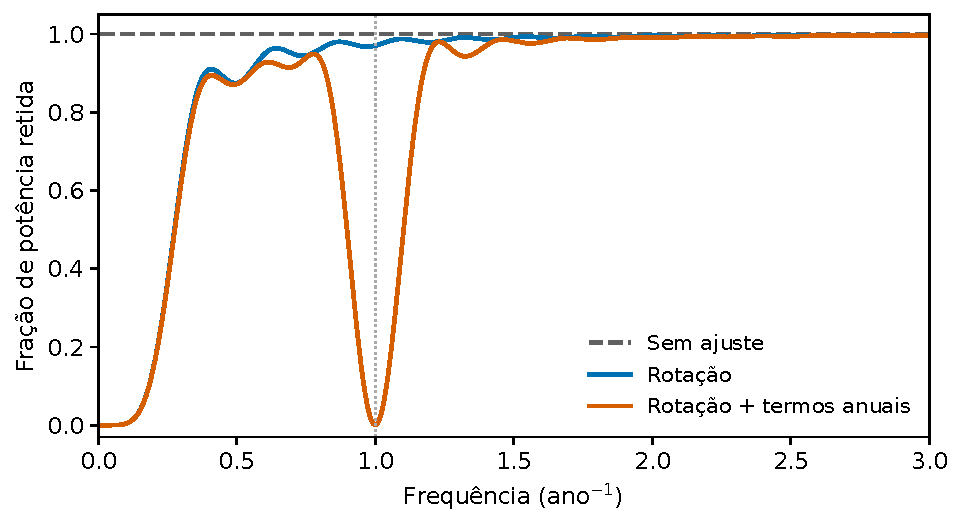
\includegraphics[width=\textwidth]{../figures/timing/transferencia.pdf}
\caption{Potência de uma senoide retida nos resíduos, em função da
frequência, com média sobre a fase inicial. O ajuste polinomial suprime
baixas frequências; os termos anuais removem a componente de período
de um ano. As curvas usam datas regulares.}
\label{fig:timing-transferencia}
\end{figure}

A Figura~\ref{fig:timing-transferencia} mostra a fração de energia
temporal retida após projetar uma senoide. A depressão anual é
consequência direta de incluir essa senoide na base ajustada.
Essa fração descreve a remoção de um sinal monocromático; a covariância
Fourier de um espectro amplo inclui também a mistura entre frequências.

\begin{figure}[htbp]
\centering
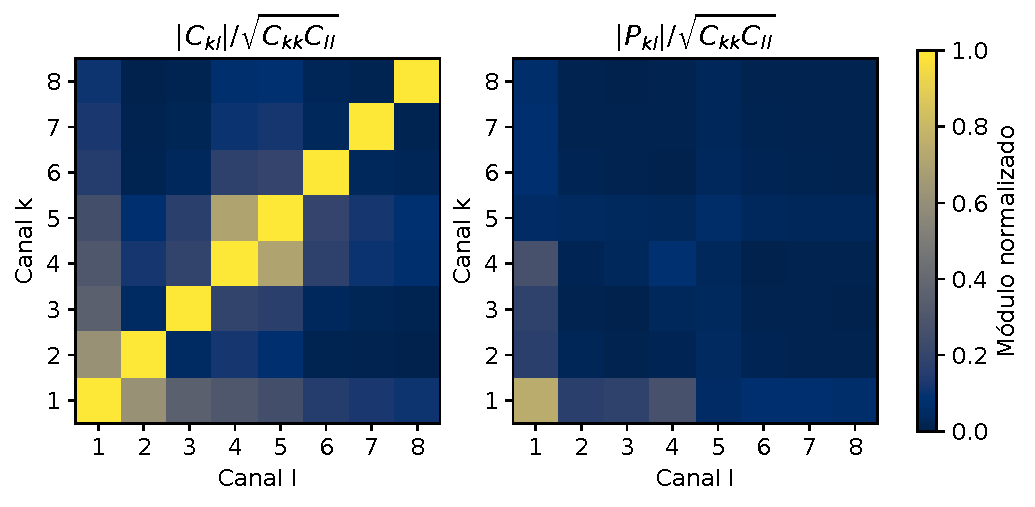
\includegraphics[width=\textwidth]{../figures/timing/covariancias.pdf}
\caption{Módulos da correlação entre canais (esquerda) e da
pseudocovariância normalizada (direita), para cadência regular com
ajuste de rotação e termos anuais. Os elementos fora da diagonal à
esquerda e os elementos não nulos à direita evidenciam a quebra das
hipóteses de independência e propriedade complexa.}
\label{fig:timing-covariancias}
\end{figure}

O efeito também pode ser expresso pela diferença entre distribuições
gaussianas. Seja $K_R$ a covariância real exata dos dezesseis
coeficientes reais e imaginários e $K_A$ a da aproximação considerada.
Para médias nulas,
\begin{equation}
 D_{\rm KL}(\mathcal N_{K_R}\Vert\mathcal N_{K_A})=
 \frac12\left[\operatorname{tr}(K_A^{-1}K_R)-16+
 \log\frac{\det K_A}{\det K_R}\right].
\end{equation}
Na grade regular com ajuste anual, conservar $C$ inteiro, mas impor
$P=0$, já produz 6,31 nat. Impor também independência entre canais
eleva a divergência para 11,22 nat. Trata-se de discrepância entre
distribuições de dados, distinta da informação posterior--priori
sobre a massa. Todas as covariâncias reais deste teste têm posto 16.

Esse experimento demonstra que a hipótese de coeficientes próprios
independentes exige verificação após o ajuste de timing. A aplicação
à massa do gráviton requer incorporar essa projeção à covariância
multípulsar, juntamente com o modelo de ruído e as datas observacionais.


\section{Extensão simulada com populações aninhadas}

\begin{figure}[htbp]
\centering
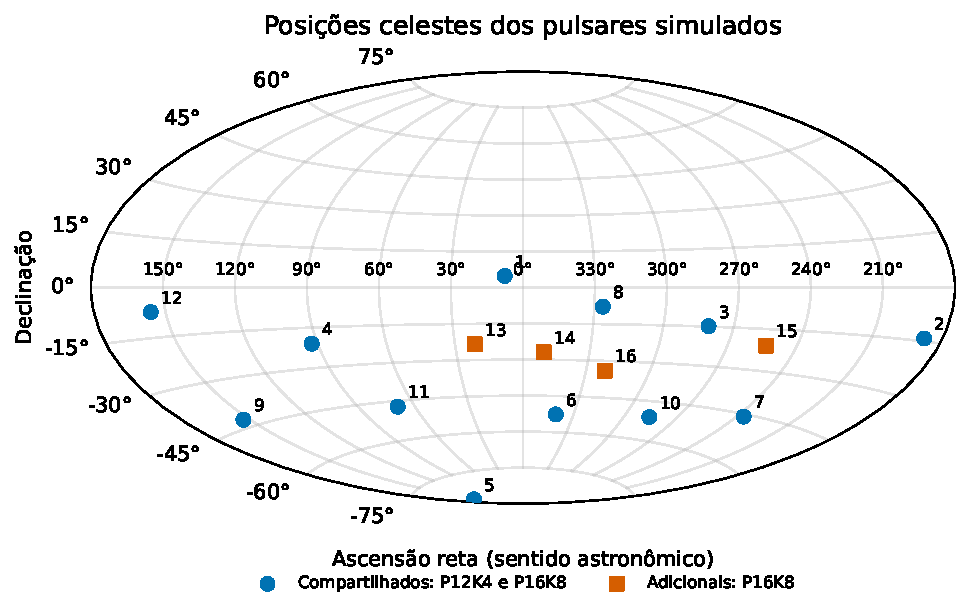
\includegraphics[width=\textwidth]{../figures/aplicacao/geometria_academica.pdf}
\caption{Direções públicas dos 16 pulsares selecionados do produto MeerKAT, com os 12 compartilhados por P12K4 e P16K8 e os quatro adicionais de P16K8. Os números correspondem à ordem determinística de seleção registrada nos metadados. Apenas as posições são observacionais: distâncias, sinais e ruídos usados no experimento são sintéticos. Fonte: metadados MeerKAT, DOI 10.57891/j0vh-5g31, CC BY 4.0; figura produzida neste trabalho.}
\label{fig:c11-geometria}
\end{figure}


O ramo executado compara P12K4 e P16K8: doze pulsares/quatro frequências e dezesseis pulsares/oito frequências. A geometria foi preparada a partir do \href{https://doi.org/10.57891/j0vh-5g31}{produto público MeerKAT}. Dos 83 PAR, 72 possuem RAJ/DECJ explícitos. Um algoritmo determinístico inicia no nome lexicograficamente primeiro e acrescenta a posição que maximiza a menor separação angular, com desempate lexicográfico. Nenhum resíduo ou resultado de inferência participa da seleção. Esse filtro de formato e a seleção angular não constituem amostra representativa da colaboração.

Os primeiros doze dos dezesseis pulsares formam o subconjunto P12. As posições públicas são tratadas como geometria fixa, sem nova solução de movimento próprio. Distâncias de 100--500 anos-luz, precisões nominais de 100--1000 ns e multiplicadores de ruído vermelho entre 0,5 e 2 são \emph{sintéticos}. Os valores dos pulsares compartilhados permanecem iguais nas duas configurações.

Ambas usam $T=4{,}5$ anos e $f_k=k/T$. Em P12K4, as dimensões são 48 coeficientes complexos em A0, 40 estimadores reais em A e 10 em B; em P16K8, são 128, 80 e 10. O máximo $fL/c$ passa de aproximadamente 397 para 889 ciclos. O último valor permanece dentro da faixa anteriormente testada na validação tensorial, e passou nos controles próprios descritos adiante. A comparação amplia simultaneamente a população e a banda; não separa causalmente o efeito de aumentar apenas uma delas.

Com nuisances conhecidos, a geração usou
\begin{equation}
 C_k(u)=P_{\rm GW}(f_k)\Gamma_k(u)+
 \operatorname{diag}\!\left[r_a^2P_{\rm red}(f_k)+2(\mathrm{EFAC}\,\sigma_a)^2\Delta t\right],
 \qquad q_k\sim\mathcal{CN}_{\rm pr\acute opria}(0,C_k).
\end{equation}
A cadência nominal é 14 dias, com $\Delta t=T/\lceil T/(14\,\mathrm{dias})\rceil$. Ela determina a potência branca do experimento periódico; não introduz uma janela real. Os parâmetros centrais são $(\log_{10}A_{\rm GW},\gamma_{\rm GW},\log_{10}A_r,\log_{10}\mathrm{EFAC})=(-15,13/3,-15{,}5,0)$, com índice vermelho individual quatro. A variável inferida é $u=f_gT$, uniforme em $[0,1]$.

A escala numérica por frequência foi comum aos canais compartilhados, usando a mediana das precisões da população 16, sem recalculá-la para P12. Nas unidades do experimento periódico, $C_k$ é uma PSD unilateral de resíduos em s$^3$, $q_k$ tem unidade s$^{3/2}$ e o coeficiente periódico é $q_k/\sqrt{2T}$. A conversão de massa é $m_gc^2=hu/T$; o suporte escolhido e seus quantis sem dados não representam uma restrição observacional.

Cada realização gerou um único vetor complexo de forma $8\times16$. P12K4 recebeu os quatro primeiros canais e os doze primeiros pulsares, sem novo sorteio. Sua covariância é a submatriz principal correspondente. Esse pareamento permite diferenças por realização, conservando a independência entre realizações de referência ou calibração.

\section{Controle gaussiano conjunto desenvolvido}

O controle G precisa preservar também a covariância cruzada entre estimadores das duas populações. Compartilhar uma semente entre duas fatorações arbitrárias não basta. Para cada frequência, escreva $C=LL^\dagger$ e $A_i=L^\dagger H_iL$. Seja $W$ uma matriz hermitiana aleatória com diagonal normal padrão real e elementos superiores $(x+iy)/\sqrt2$, com variáveis normais independentes. Define-se
\begin{equation}
 Y_i=\operatorname{tr}(H_iC)+\operatorname{tr}(A_iW).
\end{equation}
As coordenadas reais de $A_i$ na base hermitiana ortonormal são sua diagonal, $\sqrt2\operatorname{Re}A_{i,ab}$ e $\sqrt2\operatorname{Im}A_{i,ab}$ para $a<b$. Consequentemente,
\begin{equation}
 \mathbb E[Y_i]=\operatorname{tr}(H_iC),\qquad
 \operatorname{Cov}(Y_i,Y_j)=\operatorname{Re}\operatorname{tr}(H_iCH_jC).
\end{equation}
Incorporar os estimadores P12 com zeros no espaço de 16 pulsares e concatená-los aos P16 permite aplicar o mesmo vetor latente e obter a covariância conjunta correta. A construção continua válida para estimadores redundantes e uma covariância conjunta singular, sem jitter ou recorte de autovalores.

O componente foi verificado com covariâncias sintéticas: momentos, termos cruzados, orientação imaginária, estimadores nulos/duplicados e compressão linear. Uma revisão independente usou cubatura determinística em vez de repetir os sorteios do autor e encontrou erro absoluto máximo aproximadamente $1{,}60\times10^{-12}$. Esses testes verificam a álgebra do controle gaussiano; a validação da resposta física e da geração populacional é apresentada separadamente.

Os latentes CN e G usaram bancos independentes, condicionados à mesma massa. Dentro de G, A/B/C analisam o mesmo $Y$; a aproximação de resposta não altera a observação gerada. A normal conjunta reproduz os primeiros dois momentos do estimador CN, não sua distribuição inteira. A0 de P12 é marginal de A0 de P16, permitindo discutir informação esperada sob a priori; B16 e A\_G16 não determinam necessariamente os respectivos vetores P12. Não se exige ordenação dos limites superiores em realizações individuais.

\section{Desenho executado e alcance}

Foram realizadas nove análises por população: A0\_CN, A\_CN, B\_CN, C$_\beta$\_CN, C$_{\rm full}$\_CN, A\_G, B\_G, C$_\beta$\_G e C$_{\rm full}$\_G. As médias e covariâncias foram recalculadas para cada resposta. C$_\beta$ usa $\beta_1(u)=\sqrt{1-u^2}$ em todos os canais, preservando as escalas de fase $y_k=2\pi f_kL/c$; C$_{\rm full}$ usa a resposta física do primeiro canal, $\Gamma(\beta_1(u),y_1)$, em todos os canais. Ambas conservam a dependência da massa e preservam a potência e o ruído físicos. Todas as variantes de B usam a mesma observação comprimida.

O desenho prospectivo separou 500 massas da priori uniforme em $u$ de três células de 32 realizações: $u=0$ e $u=0{,}995$ com ruído central, e $u=0{,}5$ com ruído vermelho forte conhecido, $\log_{10}A_r=-14{,}7$. Os IDs 0--499 pertencem exclusivamente à calibração SBC; os 96 seguintes pertencem à recuperação condicional. A semente mestra é 20260912011, com bancos latentes independentes para CN e G e estados antes/depois de cada sorteio preservados.

Os 42 testes dos modelos corretamente especificados (A0\_CN, A\_G e B\_G, em duas populações) formam uma família Holm. Os 84 testes das aproximações formam outra, separada. Cada grupo inclui KS dos PITs de massa e logL, quatro coberturas unilaterais e a cobertura central de 90\%. O controle de multiplicidade é aplicado separadamente às duas famílias. Todas as realizações são incluídas; eventos numericamente indeterminados recebem intervalo $[0,1]$.

\section{Benchmark numérico da geometria ampliada}

O benchmark abrangeu 16 massas fixas, oito canais, duas resoluções harmônicas, oito casos independentes de integração direta no céu e seis controles de subconjunto ou rotação. As massas de referência não constituem amostra da priori para SBC.

O controle inicial identificou um erro de invariância de rotação de $4{,}58\times10^{-10}$ exclusivamente na diagonal. A recorrência de Legendre amplificava o arredondamento do produto escalar próprio. Para vetores unitários, $P_\ell(1)=1$ é uma identidade analítica; sua imposição apenas na diagonal elimina essa fonte de dependência da orientação sem alterar os termos fora da diagonal ou reparar autovalores da covariância.

O benchmark corrigido passou com diferenças máximas de $4{,}80\times10^{-12}$ entre resoluções, $6{,}14\times10^{-14}$ em relação à integração direta, $4{,}04\times10^{-12}$ nos limites analíticos e $4{,}18\times10^{-16}$ nos controles de subconjunto e rotação. Esses controles validam os nós e casos finitos examinados, não uma precisão uniforme em todo o suporte de massa.

A verificação preliminar usou 16 massas fixas nas populações P12K4/P16K8 e nove análises por população. As 288 posteriores foram comparadas entre ordens de quadratura, refinamentos independentes e representações alternativas das coordenadas, incluindo as CDFs marginais. A reconstrução dos dados apresentou desvio escalado máximo de $3{,}22\times10^{-16}$.


\subsection{Referências funcionais e campanha final}

As 18 referências diretas selecionadas antes do piloto cobrem os nove modelos nas duas configurações. Todos os quantis foram confirmados por integrais diretas em duas ordens, com respostas calculadas em duas resoluções harmônicas. Cinco eventos exigiram reduzir a massa das regiões de fronteira; as tentativas anteriores foram preservadas, sem relaxar as tolerâncias. Após esses refinamentos, os 18 controles passaram, e seus intervalos foram contidos pelos intervalos operacionais da rotina de síntese. Essa validação é finita e não prova ausência de cruzamentos em pontos não amostrados.

A rotina de síntese foi também aplicada às 288 posteriores do piloto: todas passaram nos controles de massa, enquanto 23 eventos permaneceram indeterminados e foram conservados com intervalo $[0,1]$. A campanha final foi iniciada com 500 realizações da priori uniforme em $u$ e três células de 32 realizações: $u=0$ e $u=0{,}995$ com ruído central, e $u=0{,}5$ com ruído vermelho forte conhecido. O total concluído é de 596 dados pareados e 10.728 posteriores. As famílias SBC, restritas às 500 realizações da priori, têm 42 testes de modelos corretamente especificados e 84 das aproximações, com correção Holm separada. A geração das 596 realizações foi reconstruída a partir das sementes nominais e dos estados aleatórios, com resíduo escalado máximo de $8{,}82\times10^{-16}$; o subconjunto complexo P12 foi reproduzido exatamente. A verificação reutiliza o modelo de covariância, mas reconstrói explicitamente as flutuações hermitianas e os traços quadráticos.

\section{Resultados populacionais e informação}

A comparação das duas resoluções das novas respostas apresentou diferença máxima de $4{,}80\times10^{-12}$, sustentando a precisão da resposta angular usada na população ampliada.

Os quantis de massa das 10.728 posteriores satisfizeram os critérios de precisão. Alguns conjuntos de nível de log-verossimilhança permaneceram indeterminados; seus intervalos foram propagados aos testes de calibração.

\begin{table}[htbp]
\centering
\caption{Decisões SBC da população ampliada, condicionais aos intervalos numéricos operacionais. As famílias recebem ajustes Holm separados, a 5\%.}
\begin{tabular}{lrrr}
\hline
Família & Testes & Rejeições persistentes & Indeterminadas\\
\hline
Corretamente especificados & 42 & 0 & 3\\
Aproximações & 84 & 1 & 1\\
\hline
\end{tabular}
\end{table}

A rejeição persistente ocorre no KS do PIT de logL de A\_CN em P12K4, com limite superior do valor $p$ ajustado igual a 0,004956. O teste correspondente em P16K8 é indeterminado. Nos modelos corretamente especificados, as indeterminações são os KS de logL de A0\_CN nas duas populações e de A\_G em P12K4. Ausência de rejeição persistente não comprova equivalência, nem elimina uma incerteza numérica que permite rejeição. Os testes de massa não apresentam rejeição possível nos limites adotados após Holm.

\begin{figure}[htbp]
\centering
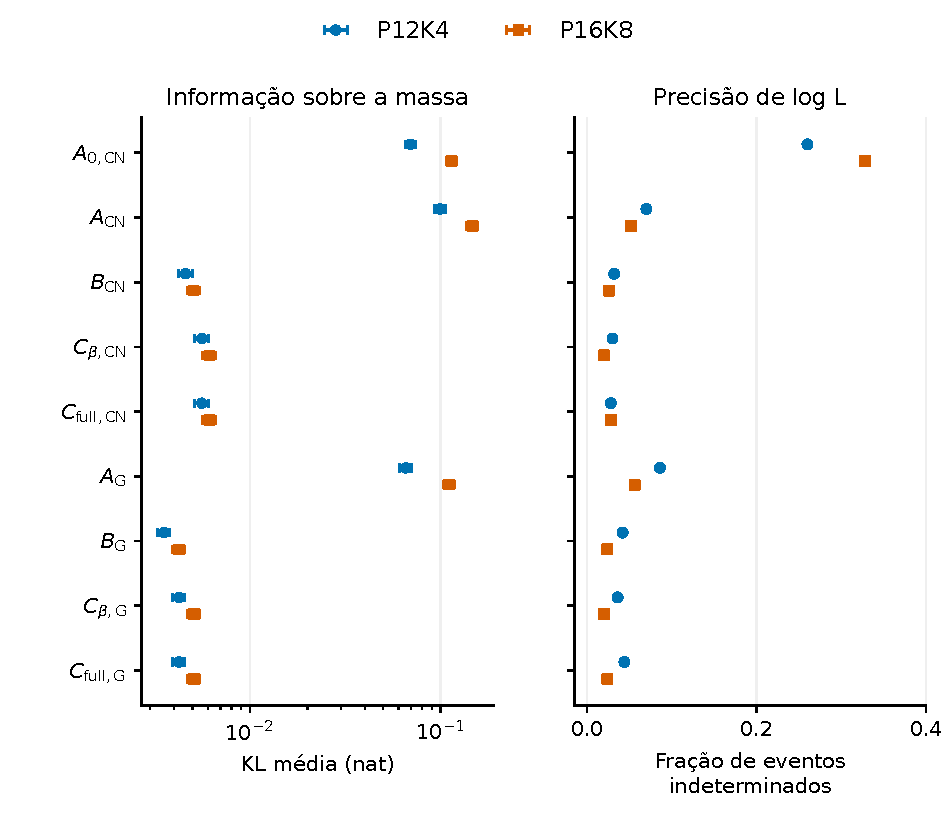
\includegraphics[width=\textwidth]{../figures/academicas/population_information.pdf}
\caption{Informação e resolução numérica nas 500 realizações da priori por grupo. À esquerda, média da divergência posterior--priori e erro Monte Carlo da média; à direita, fração de eventos de logL mantidos como indeterminados. Sob modelos aproximados, a KL é uma descrição da posterior calculada, não informação mútua do mecanismo verdadeiro. As barras não incluem erro sistemático numérico.}
\label{fig:c11-resultados}
\end{figure}

A comparação pareada A\_G menos B\_G fornece diferenças médias de KL de $0{,}06211\pm0{,}00477$ nat em P12K4 e $0{,}10631\pm0{,}00695$ nat em P16K8, onde o sinal $\pm$ indica um erro Monte Carlo da média sobre 500 realizações. Como o controle é gaussiano corretamente especificado e B é uma compressão fixa de A em cada população, essas médias estimam perda de informação esperada sob a priori. Não se exige ordenação da KL em cada realização. As 96 verdades fixas não entram nessas médias.

As posteriores comprimidas são pouco informativas neste desenho. A proximidade entre B e as variantes C pode, portanto, coexistir com pouco aprendizado sobre a massa; não autoriza usar uma resposta congelada em qualquer regime. A ampliação simultânea de pulsares e frequências tampouco identifica separadamente suas contribuições. Embora os coeficientes complexos P12 sejam subconjunto de P16, os respectivos estimadores angulares usam matrizes diferentes: não se presume que A ou B de P12 sejam compressões de A ou B de P16.

Nas três células fixas, as 32 realizações de cada modelo foram conservadas e as contagens de cobertura central foram propagadas como intervalos, com união dos intervalos binomiais. Para $u=0$, um intervalo central sob priori contínua exclui estruturalmente a fronteira; cobertura central zero nesse ponto não constitui falha de SBC nem da integração. Essas células são recuperação condicional, não amostras de calibração da priori.

\section{Precisão dos contrastes de frequência com ruído fixado}
\label{sec:contrastes-condicionais}

A comparação com marginalização dos parâmetros de ruído, apresentada
no Capítulo~\ref{chap:compressao}, deixou intervalos numéricos amplos
para as diferenças de limites superiores. Para examinar a aproximação
de frequência em uma situação mais simples, consideram-se aqui as
primeiras 50 realizações da priori da geometria de 16 pulsares e oito
frequências. A escolha dos identificadores precedeu o cálculo dos
contrastes. Os parâmetros de amplitude e ruído são fixados nos valores
de geração, e somente $u$ é integrado. A pergunta passa a ser quanto
a resposta de frequência altera o quantil de massa quando esses
parâmetros são conhecidos.

As duas representações positivas da densidade posterior, construídas
com as quadraturas de ordens 32 e 64, fornecem CDFs $F_{32}$ e $F_{64}$.
A margem de sensibilidade vertical $\varepsilon_F=0{,}002$, usada neste
capítulo, é convertida em um intervalo horizontal para o quantil:
\begin{equation}
 I_{95}=\left[
 \min_{j\in\{32,64\}}F_j^{-1}(0{,}95-\varepsilon_F),\;
 \max_{j\in\{32,64\}}F_j^{-1}(0{,}95+\varepsilon_F)
 \right].
\end{equation}
Essa inversão incorpora a inclinação local da CDF: uma mesma incerteza
vertical pode corresponder a larguras distintas em massa. Para um
contraste $Q^{(X)}_{95}-Q^{(Y)}_{95}$, o intervalo é
$[I^{(X)}_- - I^{(Y)}_+,\ I^{(X)}_+ - I^{(Y)}_-]$.
A integração independente de cada segmento polinomial por
Gauss--Legendre confirmou as 900 inversões utilizadas, com resíduo
máximo de $8{,}7\times10^{-15}$ na CDF. A incerteza relevante continua
sendo a representação da posterior, e não a solução da equação inversa.

\begin{table}[htbp]
\centering
\caption{Contrastes condicionais de $Q_{95}(u)$ nas 50 realizações.
O intervalo da média incorpora a sensibilidade numérica de todos os
pares; $r_{\max}$ é o maior afastamento de um extremo em relação ao
contraste nominal individual.}
\label{tab:contrastes-condicionais}
\small
\begin{tabular}{lrrr}
\toprule
Contraste & Média & Intervalo numérico da média & $r_{\max}$\\
\midrule
$C_{\beta,\mathrm G}-B_{\mathrm G}$ & $-0{,}000215$ & $[-0{,}004190;\ 0{,}003760]$ & $0{,}006940$\\
$C_{\mathrm{full},\mathrm G}-C_{\beta,\mathrm G}$ & $0{,}00000007$ & $[-0{,}003982;\ 0{,}003983]$ & $0{,}007122$\\
$C_{\beta,\mathrm{CN}}-B_{\mathrm{CN}}$ & $-0{,}000299$ & $[-0{,}004351;\ 0{,}003754]$ & $0{,}006927$\\
$C_{\mathrm{full},\mathrm{CN}}-C_{\beta,\mathrm{CN}}$ & $-0{,}00000029$ & $[-0{,}004064;\ 0{,}004063]$ & $0{,}007105$\\
\bottomrule
\end{tabular}
\end{table}

A sensibilidade numérica de cada contraste é inferior a $0{,}01$ em
cada direção. Para $C_\beta-B$, 49 dos 50 intervalos individuais ficam
inteiramente em $[-0{,}01;0{,}01]$, tanto no controle gaussiano quanto
nas estatísticas quadráticas físicas. Para $C_{\mathrm{full}}-C_\beta$,
essa condição vale nos 50 pares de cada família. Os intervalos das
quatro médias também cabem nessa faixa. Portanto, a aproximação produz
pequenos deslocamentos médios do limite superior nessa amostra
condicional, embora um dos pares de cada contraste $C_\beta-B$ ainda
ultrapasse a janela de equivalência.

Os intervalos da tabela descrevem a sensibilidade às representações
numéricas e à margem vertical especificada. A dispersão entre
realizações constitui outra fonte de incerteza; não foi usada aqui
para uma afirmação de equivalência populacional. Além disso, os
contrastes CN permanecem condicionais à aproximação normal da
verossimilhança. A conclusão se refere à inferência de massa com ruído
fixado nessa geometria, enquanto o efeito conjunto da aproximação e
da marginalização permanece a questão aberta do estudo anterior.


\section{Contribuição e limites da aplicação}

A extensão conecta o experimento controlado a direções reais de um catálogo, mantendo um mecanismo gerador verificável. Ela amplia os testes metodológicos anteriores e mostra, no controle gaussiano, perda de informação por compressão; também identifica um desvio persistente da aproximação normal de estimadores quadráticos em uma configuração. Isso é consistente com a distinção entre momentos corretos e distribuição correta discutida nos capítulos anteriores. Os produtos públicos verificados continuam sendo candidatos a uma aplicação observacional futura, não benchmarks observacionais reproduzidos aqui.

A aplicação a TOAs observacionais exige incorporar à posterior conjunta
de massa e ruído a projeção de timing, a cadência irregular e as
incertezas nas distâncias. O experimento da
Seção~\ref{sec:timing-sintetico} demonstra como o ajuste de rotação e
termos anuais modifica a covariância; as campanhas de inferência deste
capítulo continuam baseadas na representação periódica. Os refinamentos
e as integrações independentes sustentam as conclusões numéricas nas
configurações simuladas e fornecem referências para essa extensão.
